\subsection{Статистическая модель}
\begin{frame}
\frametitle{Модель цикла}

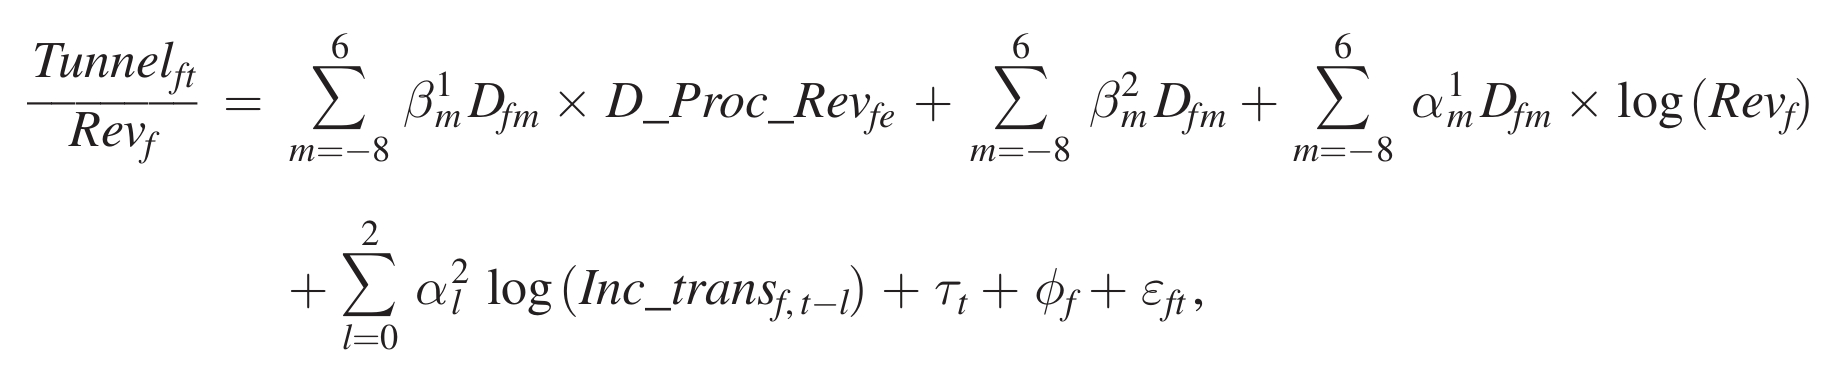
\includegraphics[scale=0.18]{images/cycle1}
\begin{itemize}
\item ...
\end{itemize}
\end{frame}

\begin{frame}
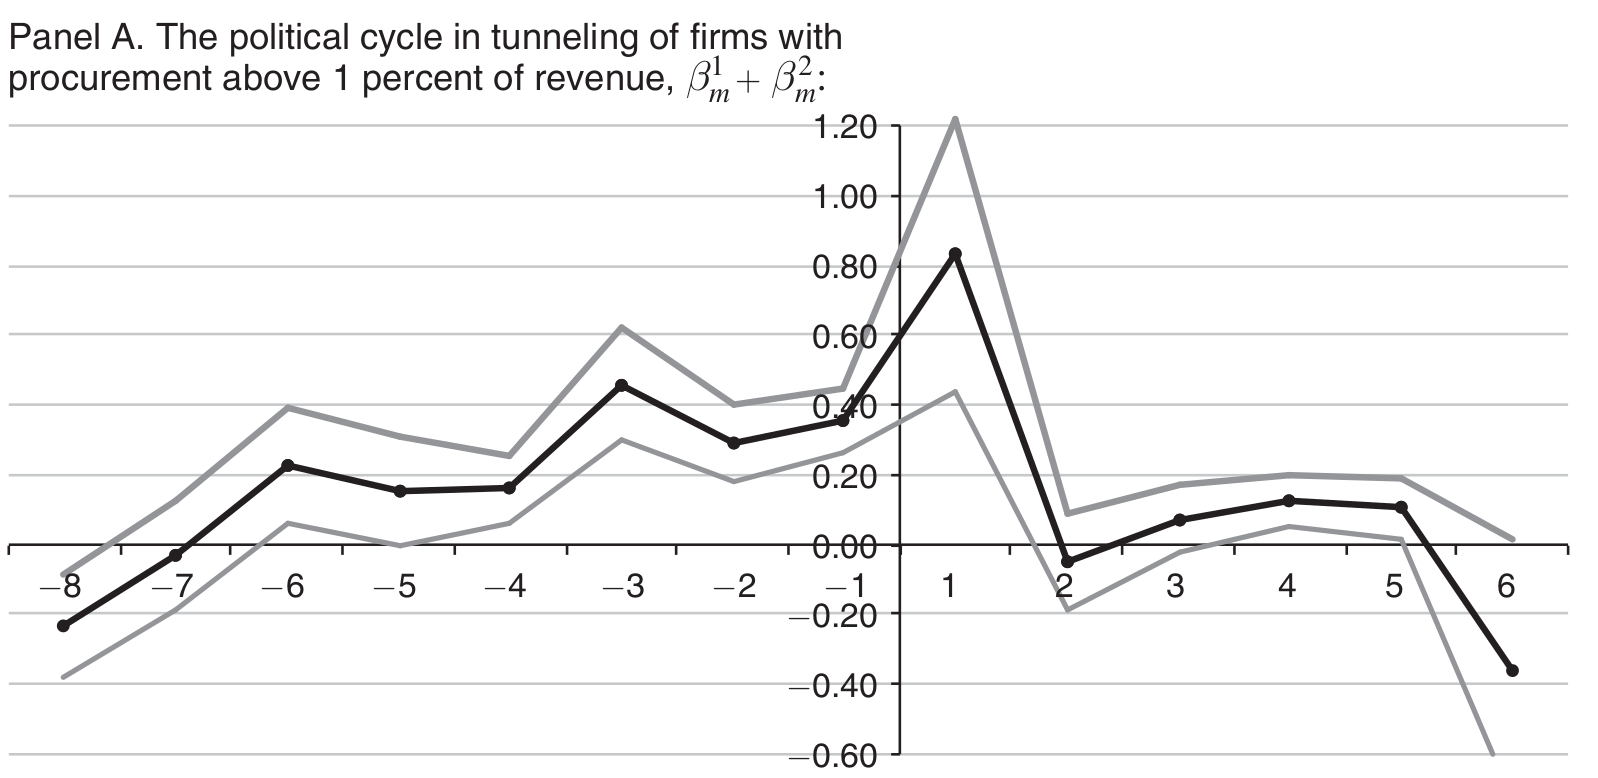
\includegraphics[scale=0.2]{images/el_effect_1}

\end{frame}

\subsection{Механизм действия}

\begin{frame}
\frametitle{Механизм влияния выборов на объем выводимых денег}
\begin{itemize}
\item Коррупция при розыгрыше тендеров:
	\begin{itemize}
	\item Необходимость подкупить действующее должностное лицо
	\item Необходимость повлиять на выборы в пользу лояльных кандидатов
	\end{itemize}

\item Увеличение экономической активности в целом, которая поднимается вследствие желания текущих должностных лиц быть переизбранными

\item Чувствительность склонности к выводу денег к доходам от гос. заказов

\item Риски, связанные с выборами - изменение политики распределения тендеров
\end{itemize}
\end{frame}
